%Oldaltorest is alkalmazhatunk
% \pagebreak
%laptores:
% \newpage


\documentclass[12pt]{report}
\usepackage[utf8]{inputenc}
\usepackage[T1]{fontenc}
\def\magyarOptions{defaults=hu-min}
\usepackage[magyar]{babel}

\usepackage{times}
\usepackage{tcolorbox}

\usepackage{amsmath}
\usepackage{amssymb}
\usepackage{amsthm}

\usepackage{fancyhdr}

\usepackage{graphicx}
\usepackage{psfrag}

\usepackage{setspace}
\usepackage{float}
\usepackage{hyperref}

\graphicspath{ {images/} }

%Margok:
\hoffset -1in
\voffset -1in
\oddsidemargin 35mm
\textwidth 150mm
\topmargin 15mm
\headheight 10mm
\headsep 5mm
\textheight 237mm

% \onehalfspacing
\linespread{1.25}

\begin{document}


\thispagestyle{empty}

\begin{center}
{\Large\bf Szegedi Tudományegyetem}

\vspace{0.5cm}

{\Large\bf Informatikai Intézet}

\vspace*{8.5cm}


{\Huge\bf SZAKDOLGOZAT}


\vspace*{7cm}

{\LARGE\bf Kovács-Bodó Csenge}

\vspace*{0.6cm}

{\Large\bf 2024}

\end{center}

\newpage


\fancypagestyle{plain}{
\fancyhf{}
\fancyfoot[R]{\thepage}
\renewcommand{\headrulewidth}{0pt}
}


\pagestyle{fancy}
\fancyhf{}
\fancyhead[L]{Beszédfelismerő és képernyő felolvasó játék fejlesztése vakok és látássérültek számára}
\fancyfoot[R]{\thepage}


\thispagestyle{empty}

\begin{center}
\vspace*{1cm}
{\Large\bf Szegedi Tudományegyetem}

\vspace{0.5cm}

{\Large\bf Informatikai Intézet}

\vspace*{3cm}


{\LARGE\bf Beszédfelismerő és képernyő felolvasó játék fejlesztése vakok és látássérültek számára}


\vspace*{3cm}

{\Large Szakdolgozat}

\vspace*{3cm}

{\large
\begin{tabular}{c@{\hspace{4cm}}c}
\emph{Készítette:}     &\emph{Témavezető:}\\
\textbf{Kovács-Bodó Csenge}  &\textbf{Dr. Jánki Zoltán Richárd}\\
Gazdaságinformatikus         &Egyetemi adjunktus\\
BSc hallgató&\\
\end{tabular}
}

\vspace*{1.5cm}

{\Large
Szeged
\\
\vspace{2mm}
2024
}
\end{center}

\renewcommand{\contentsname}{Tartalomjegyzék}

\chapter*{Feladatkiírás}
\addcontentsline{toc}{section}{Feladatkiírás}

Az esélyegyenlőség jegyében már számos program elérhető az interneten, melyeket kifejezetten vakok és látássérültek számára készítettek el, emellett nagy népszerűségnek örvend általános felhasználók körében is, ha egy program felhasználói ferülete minél könnyebben használható, felhasználóbarát. Szakdolgozatom célja olyan frontend oldali technológiák, módszerek tárgyalása, melyekkel akadálymetesíthetünk egy programot látásukban korlátozott felhasználók számára. Példa proramom egy egyszerű memóriajátékok mutat be, melyet hangvezérléssel irányíthatunk, és a program folyamatos szövegfelolvasással visszajelzést küld és segít a tájékozódásban.

\chapter*{Tartalmi összefoglaló}
\addcontentsline{toc}{section}{Tartalmi összefoglaló}

\textbf{A téma megnevezése:} \\
\noindent Beszédfelismerő és képernyő felolvasó játék fejlesztése vakok és látássérültek számára\\

\noindent\textbf{A megadott feladat megfogalmazása:} \\
\noindent Szakdolgozatom célja olyan módszerek és technológiák bemutatása, amelyekkel vakok és látássérültek számára kényelmesen használható, kiváló felhasználói élményt nyújtó játékot készítek. \\

\noindent\textbf{A megoldási mód:} \\
\noindent Az alkalmazás célja, hogy a felhasználók billentyűzet és egér nélkül, akusztikus módszerekkel irányíthassák a játékot, mivel nem támaszkodhatnak a látásukra. Ehhez a Web Speech API beszédfelismerő és beszédszintetizáló funkcióit használtam, melyeket a program egyes részein felüldefiniáltam. \\

\noindent\textbf{Alkalmazott eszközök, módszerek:} \\
\noindent A demonstrációs projekt a legújabb Angular keretrendszerrel készült. Létrehoztam egy Firebase projektet, amelyben Firestore-t használtam a játék eredményeihez, Storage-t a kártyák képeinek tárolására, és Hostingot a program kitelepítéséhez. A beszédfelismerést és szintetizációt a Web Speech API két interfészével valósítottam meg. \\

\noindent\textbf{Elért eredmények:} \\
\noindent Létrehoztam egy webes memóriajátékot, amelyhez nem szükséges billentyűzet vagy egér, mert hangparancsokkal irányítható, és beszédszintetizációval ad visszajelzést. Az egér mozgatásával az alkalmazás felolvassa a szövegeket és elemek nevét. A játék magyar vagy angol nyelven is játszható, testreszabható beállításokkal. Van egyszemélyes és kétszemélyes mód, az egyéni eredmények pedig ranglistára küldhetők. \\

\noindent \textbf{Kulcsszavak:} \\
\noindent beszédfelismerés, beszédszintetizáció, szövegfelolvasás, Web Speech API

\tableofcontents

\chapter*{Bevezetés}
\addcontentsline{toc}{section}{Bevezetés}

Vakok és látássérült emberek számára elérhető eszközök, játékok, könyvek vagy alkalmazások tervezése és készítése napjaink legnagyobb kihívása, viszont az egyik legszebb feladata. Fontos missziója a társadalmunknak ezen emberek integrálása, befogadása közösségünk közé. A testileg vagy szellemileg sérült emberek gyakran szembesülhetnek azzal, hogy a piacon található alkalmazások nem megfelelő számukra, emiatt kirekesztettnek érezhetik magukat, önbecsülésük csökken, szociális készségeik visszamaradottak. Középiskolában volt egy osztálytásam, aki egy ritka szembetegséggel született, ennek eredményéül maximum 10 százalékot látott a külvilágból. Nehezen nyitott mások felé, nehezen tudott tanulni, lassan írt kézzel viszont gépelni egyáltalán nem tudott.

\noindent
A technológia rohamszerű fejlődésének köszönhetően már számos olyan könyvtár elérhető, amit a legtöbb magaszsintű programozási nyelv is keretrendszer támogat. Az elmúlt évtizedben nagy hangsúlyt fektettek a fejlesztő cégek olyan szoftverek értékesítésébe, melyben különféle akadálymentesítést szolgáló funkciók elérhetőek, és a felhasználói élményt maximalizálták.

\noindent
Szakdolgozatom célja ezen technológiák, frontend fejlesztési alapelvek, módszerek ismertetése, összegyűjtése, melyekkel vakoknak, látássérültek és színvakoknak is egyaránt tudunk szoftvereket tervezni és fejleszteni. Példaprogramom egy olyan memóriajátékot mutat be, melyben nem szükséges a látásunkra hagyatkozni, illetve billentyűzetre és egérre sem lesz feltétlen szükség, hanem akusztikus módszerekkel tudjuk kezelni az alkalmazást, mégpedig úgy, hogy az a felhasználó szóban kiadott parancsokkal tudja irányítani az egész programot, tehát a játék beszédfelismerésre képes, eközben szövegfelolvasással és beszédszintetizációval segít az oldalon való könnyeb tájékozódásban.

\chapter{Terület áttekintése, jelenleg ismert technológiák}
Már egyre több új szoftver, létező alkalmazásokban új funkciók elérhetőek a piacon, melyeket kimondottan vakoknak, látássérültek vagy színvakok számára fejlesztettek. Ezek közül bemutatom a legnépszerűbbeket.
\section{Apple VoiceOver}
A VoiceOver \cite{voiceover} egy fejlett képernyőfelolvasó funkció Mac Os X operációs rendszerekben, mely lehetővé teszi látássérült felhasználók számára, hogy könnyedén vezérelhessék telefonjukat, táblagépüket vagy számítógépüket billentyűzetparancsokkal \cite{keysforvoiceover} és gesztusokkal. \cite{usingvoiceover} A képernyő tartalmában szakaszosan tud lépegetni a felhasználó, miközben a készülék automatikusan felolvassa a képernyő tartalmát. Mac gépeken a Command-F5 billentyűkombinációval kapcsolható be, Iphone-okon és Ipad-eken a beállításokon belül a kisegítő lehetőségek menüpontban található, vagy Siri-nek kiadott utasítással is bekapcsolható. A Braille kijelzők \cite{braille} és a Multi-Touch trackpad \cite{multitouch} megjelenése óta már egyszerű kézi gesztusokkal is vezérelhető a felolvasás. \cite{usingvoiceover}

\section{Intelligens személyi asszisztens}
A VoiceOver-nél említett Siri \cite{siri}, Samsung eszközökön a Bixby \cite{bixby}, Amazon Alexa és Alice mind-mind olyan intelligens személyi asszisztens program okoseszközökön, mely nagy mértékben egyszerűsíti és gyorsítja eszközeink használatát. Elég egyetlen szóban kiadott utasítás és a program a felhasználó helyett elvégzi az eszközön a feladatot, például hívást indít, rákeres bármire a böngészőben, megnyitja a letöltött applikációkat. Ez a funkció rendkívül hasznos látássérülteknek, mivel egyáltalán nem kell a kezüket használni okostelefonjuk kezeléséhez.

\section{SciFY}
A SciFY (Science For You) \cite{scify} egy görög nemzetközi szervezet, mely ingyenes és nyílt forráskódú LEAP (Listen - LEArn - Play) játékokat fejleszt kifejezetten vakok és gyengénlátó gyermekek számára. A játékok célja, hogy segítsenek a gyerekeknek új készségek elsajátításában, miközben szórakoztatják őket. Hivatalos weboldalukon, a \linebreak \url{https://gamesfortheblind.org} oldalon különböző játékokat található, mint például a Tic Tac Toe, Tennis és Curve, amelyek különböző nehézségi szinteken játszhatók. Ezek a játékok háromdimenziós binaurális hanggal rendelkeznek, amelyeket a játékosok teljes mértékben kihasználhatnak. A weboldalon kívül a Memor-i Online platformon bármelyik felhasználó könnyedén létrehozhat saját, inkluzív memória játékot, amelyet akár vak, semleges vagy látó játékosok is játszhatnak. A platform célja, hogy lehetővé tegye a vak és látó gyermekek közötti együtt játszást, és segítse a gyerekek fejlődését

\section{Chrome-ban támogatott bővítmények és csomagok}
Fellehető egy kiváló leírás a Google Codelabs jóvoltából a \linebreak \url{https://codelabs.developers.google.com/angular-a11y#0} oldalon, ahol pontokba szedve adnak tippeket, hogyan lehet egy Angular-ban írt felhasználó felület minél jobban akadálymentesített, mire figyeljen egy fejlesztő, mikor színvakoknak tervez alkalmazást. Egy egyszerű képernyőolvasó módszert is bemutat, melynek lényege, hogy a HTML elemeinket felcímkézzünk ARIA label-ökkel, ahol megadjuk, hogy a program mit olvasson fel, majd egy Chrome Web Store-ból letöltjük a megfelelő bővítményt \cite{chromevox}, amely felolvassa a label-ök tartalmát.

\pagebreak
Példa egy ARIA label-el felcímkézett Angular Material elemre\cite{ariaex}:

\begin{verbatim}
    <mat-slider
      aria-label="Dumpling order quantity slider"
      id="quantity"
      name="quantity"
      color="primary"
      class="quantity-slider"
      [max]="13"
      [min]="1"
      [step]="1"
      [tickInterval]="1"
      thumbLabel
      [(ngModel)]="quantity">
    </mat-slider>
\end{verbatim}
\newline
További akadálymentesítést elősegítő bővítmények: Chrome Web Store-ban \cite{extensions}.

\section{Referencia alkalmazások}
Példaprogramom fejlesztése előtt áttekintettem valamennyi nyílt forráskódú programokat, publikus GitHub repository-kat \cite{web-speech-angular}\cite{pacman}\cite{audio-games}, melyek beszédfelismeréssel és beszédszintetizációval működnek. A kiválasztott technológia, amivel elkészítettem a játékot, a Web Speech API, mely egy követekző fejezetben bemutatásra kerül.

\chapter{A program funkcionális specifikációi}
\section{Funkcionális elvárások}
A szakdolgozatomhoz elkészített szoftver egy olyan játékot mutat be, amely a Web Speech API SpeechRecognition és SpeechSynthesis részAPI-jait használja, tehát ismerje fel a felhasználó által adott verbális utasításokat, majd dolgozza fel őket a teljes weboldalon, emellett adjon rendszeres visszajelzést szóban a felhasználónak beszédszintézissel.
\newline
A weboldal megnyitásakor a felhasználó kiválaszthatja, hogy magyarul, vagy angol nyelven szeretné használni az alkalmazást, és a program eszerint le lesz fordítva.
\newline
A program egy egyszerű memóriajátékot mutat be, melyet egyedül és párban is lehet játszani. Egyszemélyes játékban pontokat lehet gyűjteni időre. Sikeres játék végén egy becenévvel felkerülhet a játékos egy globális ranglistára.
\newline
Elérhető egy beállítások menü, ahol a játékos személyre szabhatja a játék méretét, időtartamát, beállíthatja, hogy egyszemélyes vagy kétszemélyes játékkal szeretne játszani, illetve a program hangerejét és lejátszási sebességét is megváltoztathatja.
\newline
A játék mögött áll egy Firebase alkalmazás, mellyel eltároltam a kártyák képeit és a ranglista adatait, illetve kitelepítettem publikusan a Webre a Hosting szolgáltatással.
\pagebreak
\section{Használati eset diagram}
\noindent
A program használati esetei a nyelv kiválasztása, a játék személyre szabhatósága és használata, illetve az eredmények tárolása Firebase adatbázisban. Ezeket az eseteket mutatja be az alábbi ábra.
\begin{figure}[H]
  \centerline{\includegraphics[scale=.75]{usecase.eps}}
  \caption{Use case diagram}
\end{figure}
\pagebreak
\section{Szekvenciális diagram}
\noindent
Az alábbi ábra bemutatja a program legfontosabb folyamatait, hogy hogyan jut el a felhasználó program megnyitásától a játék eredményeinek tárolásáig. A eljárások során a játékos végig képes hangutasításokat kiadni és a program beszédszintézissel válaszol.
\begin{figure}[H]
  \centerline{\includegraphics[scale=.75]{sequence.eps}}
  \caption{Szekvenciális diagram}
\end{figure}
\linebreak
\noindent
A használati esete és szekvenciális diagramokat a draw.io programmal készítettem el.\cite{drawio}
\pagebreak
\chapter{Használt technológia-A Web Speech API}
\section{Gépi beszédfelismerés háttere}
A számítógépes beszédfelismerés \cite{infu} egy összetett folyamat, amely az emberi beszéd digitális feldolgozásán alapul, hogy azt a számítógép írott formába alakítsa. Az alábbiakban a legfontosabb elemeket és alapelveket foglalom össze, érthető formában.
\subsection{Alapfogalmak: Az osztályozási feladat}
A beszédfelismerés olyan osztályozási probléma, ahol a cél az, hogy adott hangokról eldöntsük, melyik fonémához (beszédhanghoz) tartoznak. Ehhez a hangokat számítógéppel feldolgozva, jellemzőkkel (adatokkal) írjuk le. Az osztályozás Bayes-döntéselmélet alapján történik, amely azt mondja ki, hogy az a döntés optimális, amelyik a legvalószínűbb kimenetet választja az adatok alapján.
\subsection{A statisztikai módszerek kihívásai}
A statisztikai alapú megközelítés során gyakran két fő probléma merül fel:
\begin{itemize}
    \item Adatkorlátok: Kevés példa esetén a statisztikák pontatlanok lehetnek.
    \item Dimenziós problémák: Sok jellemző és lehetséges kombináció mellett az adatok feldolgozása exponenciálisan nehezebbé válik.
\end{itemize}
\pagebreak
Lehetséges megoldások:
\begin{itemize}
    \item Több adat gyűjtése.
    \item A jellemzők számának csökkentése, azaz kizárólag a releváns adatok használata.
    \item A valószínűségek egyszerűsítése (például az egyes jellemzők függetlenségét feltételezve).
\end{itemize}
\subsection{A beszédfelismerő rendszer felépítése}
A tipikus beszédfelismerő rendszer több modulból áll:
\newline
\raggedright\textbf{a) Előfeldolgozás:}\linebreak
A beszédet digitális jellé alakítják, amelyet spektrogram formájában elemeznek. Ezt követően csökkentik az adatmennyiséget, például a kevésbé fontos részek eltávolításával.
\newline
\raggedright\textbf{b) Akusztikai-fonetikai modell:}\linebreak
Ez a rész a hang és a beszédhangok (fonémák) közötti kapcsolatot térképezi fel. Ehhez gyakran rejtett Markov modelleket (HMM-eket) használnak, amelyek a beszédet kisebb egységekre bontva értékelik.
\newline
\raggedright\textbf{c) Nyelvi modell:}\linebreak
Ez a modul a lehetséges beszédkombinációk valószínűségét határozza meg. Például az angol nyelvben a szavak előfordulási valószínűségét, míg magyarban a ragozási szabályokat figyelembe véve működik.
\newline
\raggedright\textbf{d) Dekóder:}\linebreak
Ez az egység összevonja az előző modellek eredményeit, hogy az egész beszédet szöveggé alakítsa. A folyamat során számos hipotézist vizsgál meg, és a legvalószínűbbet választja ki.
\linebreak
Tehát megállapítható, hogy a számítógépes beszédfelismerés lényege, hogy az emberi beszédet digitális jelekké alakítja, és statisztikai, valamint gépi tanulási módszerek segítségével fonémákra, majd írott szövegre fordítja. A módszerek fejlesztésének kulcsa az adatok pontos feldolgozása és a modellek folyamatos finomítása.
\pagebreak
\section{A Web Speech API}
A Web Speech API \cite{webspeechapi} egy böngésző alapú API, amely lehetővé teszi beszéd alapú alkalmazások létrehozását webfejlesztők számára. Ez az API különösen hasznos a látássérült felhasználók számára, vagy azoknak az alkalmazásoknak, amelyek interaktívabb élményt szeretnének nyújtani. Két fő eleme:
\begin{itemize}
    \item SpeechRecognition:
    \begin{itemize}
	   \item lehetővé teszi a weboldalak számára, hogy felismerjék és feldolgozzák a felhasználó beszédét. Ez hasznos lehet például hangalapú keresésekhez vagy hangvezérelt feladatokhoz.
    \end{itemize}
    \item SpeechSynthesis:
    \begin{itemize}
	   \item lehetővé teszi, hogy a program beszéljen egy adott nyelven. Például, ha egy weboldal szeretne szöveget felolvasni, a SpeechSynthesis segítségével ezt megteheti.
    \end{itemize}
\end{itemize}
\newline
Használata kizárólag JavaScript-ben biztosított, ezen két funkció a SpeechSynthesisUtterance és a SpeechRecognition objektumok használatával érhető el.\cite{usingwebspeechapi}

\subsection{SpeechRecognition}
A SpeechRecognition \cite{speechrecognition} API a Web Speech API része, amely segítségével webalkalmazások képesek felismerni és feldolgozni a felhasználók beszédét. Az API lehetővé teszi a beszédfelismerési folyamat indítását, amely során a mikrofonon keresztül érkező hangokat elemzi és szöveggé alakítja. Számos eseményt kínál, mint például onresult, onspeechstart, onspeechend, amelyekkel a fejlesztők különböző eseményeket kezelhetnek a felismerési folyamat során. Támogatja a folyamatos felismerést is, ahol a beszédfelismerés nem áll le az első mondat után, hanem folytatódik, amíg a felhasználó beszél.
\newline
Támogatottsága böngészőnként eltérő lehet, jelenleg Safari-ban még nem támogatott. Emellett biztonsági kockázatokkal is járhat a mikrofon engedélyezése. Bármely program inicializálásakor a felhasználó dolga mikrofonjának engedélyezése a böngészőnek, ennek hiányában nem fog működni a beszédfelismerés.
\pagebreak
Példa kód:
\begin{verbatim}
var recognition =
new (window.SpeechRecognition || window.webkitSpeechRecognition)();
recognition.lang = 'hu-HU'; recognition.continuous = true;
recognition.interimResults = false;
recognition.onresult = function(event) {
    var transcript = event.results[0][0].transcript;
    console.log(transcript);
};
recognition.start();
\end{verbatim}

\subsection{SpeechSynthesis}
A SpeechSynthesis \cite{speechsynthesis} API a Web Speech API része, amely lehetővé teszi, hogy egy weboldal beszédfelismerést és beszédszintetizációt valósítson meg, ezzel akár saját képernyőolvasó funkciót is implementálhatunk. Az API szöveget alakít hanggá és lejátssza felhasználóknak. Személyre szabhatjuk a szintetizált beszéd tulajdonságait, mint nyelvét, a beszéd sebességét, hangmagasságát és hangerejét. A SpeechSynthesisUtterance objektum tartalmazza a szintetizált beszéd szövegét és beállításait és a SpeechSynthesis objektum vezérli a beszédszintetizálási szolgáltatást, például elindítja vagy leállítja a beszédet. Legfontosabb függvénye a speak(), mely két paramétert vár: a kimondandó szöveg és a nyelv.

Példa kód:
\begin{verbatim}
    var msg = new SpeechSynthesisUtterance();
    msg.text = "Heló Világ!";
    //msg.lang = "hu-HU" // Nyelv
    msg.volume = 1; // Hangerő
    msg.rate = 1; // Lejátszási sebesség
    msg.pitch = 1; // Hangmagasság
    window.speechSynthesis.speak(msg, "hu-HU");
\end{verbatim}
\pagebreak
\chapter{A program megvalósítása}
Ebben a fejezetben bemutatom a szakdolgozat példaprogramjának megvalósítását, a tervezéstől a kivitelezésig.
\section{A program architektúrája}
Szakdolgozati szoftverként egy Angular CLI alkalmazást készítettem el. A jelenleg legfrissebb, 17.3.0-s verzióju Angularral fejlesztettem, 20.12.1-es Node.js-sel és 10.5.0-s verzióju Node Package Managerrel. A program teljes logikáját a komponensek TypeScrip file-jaiban írtam meg, néhány service-szel kiegészítve, nem kötöttem hozzá másik backend programot.
\newline
Az alkalmazás számos komponensből épül fel, melyek a következők:
\begin{itemize}
    \item AppComponent: a program magja, ebből indul ki a többi komponens, kivéve a SetlanguageComponent, és adjuk át a service-eknek az alkalmazás nyelvét.
    \item HomepageComponent: a főoldal komponense.
    \item HelperComponent: egy segítség dialógus, amely felolvassa az összes olyan utasítást, amelyeket a felhasználó ki tud adni, hogy irányíthassa a programot.
    \item GameComponent: egyszemélyes játék komponense. Egy egyszerű memóriajátékkal tudunk játszani, mely méri az időnket és gyűjti a pontokat.
    \item SuccessComponent: egy dialógus ablak, amely akkor jelenik meg, ha megtaláltuk az idő letelte előtt az összes párt. Itt megadhatjuk a nevet amivel szeretnék szerepelni a ranglistán és elküldjük az eredményeket a Firestore-ba.
    \item RetryComponent: egy dialógus ablak, amely akkor jelenik meg, ha nem találtuk meg az összes párt. Innen új játékot lehet kezdeni.
    \item RankingsComponent: a korábbi eredményeket listázza ki a Firestore-ból rangsorolva pont- és idő alapján.
    \item SetlanguageComponent: a weboldal megnyitásakor mindig ez a komponens jelenik meg. Itt állítjuk be a szoftver nyelvét.
    \item SettingsComponent: a beállítások menü komponense, mely az alábbi almenüket tartalmazza:
    \begin{itemize}
        \item BoardsizeComponent: játékméret beállítása. Háromszor négyes, Négyszer négyes és négyszer ötös méretek elérhetőek.
        \item NumberofplayersComponent: játékosok számának beállítása. Egyszemélyes és kétszemélyes játék közül lehet választani.
        \item TimeComponent: játékidő beállítása. 60, 120, 180 vagy 300 másodperc állítható be.
        \item VolumeandspeedComponent: itt a hangerő és a lejátszási sebesség állítható be.
    \end{itemize}
    \item MultiplayerComponent: kétszemélyes játék komponense. Nem méri az időt és a pontokat, kizárólag a két játákos talált párjainak a számát.
    \item MultiplayersuccessComponent: ez a dialógus akkor jelenik meg, ha megtalálták az összes párt. Kiírja, illetve felmodja a nyertes nevét, vagy ha döntetlen lett az állás.
\end{itemize}

Valamint az alábbi service-ekből:
\begin{itemize}
    \item CardService: kártyák betöltése Storage-ból
    \item GameService: segít a játék és a beállítás menü között a játék tulajdonságainak a kezelésében.
    \item LanguageService: kommunikál a SetlanguageComponent és a többi komponens között, beállítja nyelvet.
    \item SpeechRecognizerService: a beszédfelismerésért felelős service.
    \item SpeechSynthesizerService: a beszédszintézisért felelős service.
    \item VoiceoverService: a képernyőolvasást megvalósító service.
\end{itemize}
\pagebreak
Mivel a böngésző az operációs nyelv beállított, illetve letöltött nyelvi csomagjait tudja használni a Web Speech API használatához, így nagyon fontos, hogy az alkalmazás használata előtt azokat a nyelveket, melyeket használni szeretnénk a programban, az operáció rendszer nyelvi beállításaiban töltsük le a megfelelő nyelvi csomagokat. Alapértelmezetten támogatott minden operációs rendszerben az angol nyelv, viszont a magyar nyelv nem, ezért különösen fontos a felhasználóknak erről gondoskodniuk.
\section{Adatmodellek}
Három fő adattal dolgoztam az alkalmazás fejlesztése során. A program elején beállítottam a nyelvet, melyet egy string-ként átadtam a beszédfelismerését és a beszédszintéziésért felelős service-eknek. Amennyiben magyar nyelvet választ ki a játékos, a "hu-HU", angol nyelv esetén a "en-US" string kerül átadásra. A játékban használt kártyákat nem a program repository-jában tároltam el, hanem az alkalmazás mögött álló Firebase Storage-ában. A képeket a Storage-ból az elérési útvonaljukkal (string) és egyedi Access token-jük (string) segítségével értem el. A képek betöltéséhez készítettem egy service-t CardService néven.
\newline
\newline
Kártyák betöltése Storage-ból:
\begin{verbatim}
  getImage(imageUrl: string){
    return this.storage.ref(imageUrl).getDownloadURL()
  }
\end{verbatim}
\newline
Ez a metódus a játék során betölti azt annak kártyának a képét, melyet kiválasztott a játékos. Paraméterben megkapja a kép elérési útvonalat (esetünkben a cards/ mappából), a this.storage.ref(imageUrl) segítségével létrehoz egy hivatkozást a Firebase Storage-ban található fájlhoz, majd a getDownloadURL() metódust hívja meg a hivatkozáson, amely egy Promise-t ad vissza, mely tartalmazza a képeket.
\pagebreak
A kártyák elérési útvonalát egy konstansban tároltam el.
\begin{verbatim}
    export const cardpictures  =[
      "cards/cat.png",
      "cards/ball.png",
      "cards/candy.png",
      "cards/car.png",
      "cards/cloud.png",
      "cards/dog.png",
      "cards/flow.png",
      "cards/rose.png",
      "cards/sun.png",
      "cards/umb.png"
    ]
\end{verbatim}

Végezetül a játék során eltároljuk az eredményeket a ranglistába. Az adatokat a Firebase app Firestore-jába mentjük el, a rankings kollekcióba:
\begin{itemize}
    \item documentId(string): egyedi azonosítója a Firestore dokumentumnak, amely egy rangsori helyezés adatait tárolja
    \item name(string): felhasználónév(felhasználói inputról)
    \item points(number): a játék során elért pont
    \item time(number): a játékban eltöltött másodpercek száma
    \item date(timestamp): a játék adatainak mentési ideje(mm dd, yy at hh:mm:ss AM/PM timezon formátumban)
\end{itemize}
Az adatok kezeléséhez készítettem egy TypeScript interfészt is.
\begin{verbatim}
    export interface Ranking{
     name:string;
     points: number;
     time: number;
     date: any;
    }
\end{verbatim}
\section{Verziókövetés}
A fejlesztési folyamat során a programot a kezdetektől a befejezésig verziókövetéssel kezeltem a GitHub platformon, biztosítva a kód folyamatos nyomon követhetőségét és dokumentáltságát. A végleges alkalmazást a Firebase Hosting szolgáltatás segítségével deploy-oltam, amely stabil és megbízható környezetet biztosított a projekt publikálásához. A \url{https://blindmemorygame-szakdolgozat.web.app/} címen publikusan elérhető bármely böngészőben az alkalmazás.

\section{A játék grafikus interfészének elkészítése, jellemzői}
A szoftver felhasználó felületének elkészítése során különös figyelmet szenteltem arra, hogy színvakok számára megfelelő legyen. Figyelmet fordítottam a színekre, nem használtam olyan kombinációk, melyeket színtévesztők könnyen összekeverhetnek, mint például a piros és zöld együttese. Egy sötétkék háttért választottam, és a szövegeket fehérre színeztem, hogy minél kontrasztosabb legyen. Átlagosan 60 pixel nagyságú betűméretet  sans-serif betűtípust adtam meg a css file-okban, amely egy talpatlan betűtípus, ezáltal könnyebben olvasható. Minden gombot, toggle csúszkát, görgetős elemet és ikont a lehető legnagyobb méretűre állítottam. Az elért eredményem pedig, hogy a Developer Tools minden elememre pipát írt a Contrast értékre, amely azt mutatja, hogy könnyen olvasható, akadálymentesített a felület.
\begin{figure}[H]
  \centerline{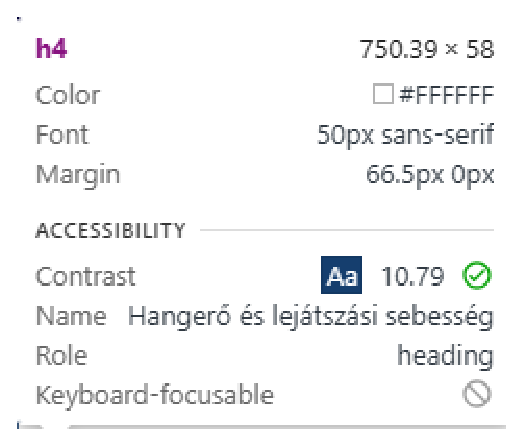
\includegraphics[scale=1]{accessible.eps}}
  \caption{Vizsgálat Developer Tools-ban egy tetszőleges elemre.}
\end{figure}
\section{Beszédfelismerés implementálása}
\section{Beszédszintetizáció impementálása}
\section{Képernyőolvasás implementálása}
\pagebreak
\section{Angol-és magyar nyelvre fordítás implementálása}
Annak érdekében, hogy elkerüljem a magyar és angol szövegek közvetlen beleégetését a HTML és TypeScript kódokba, kidolgoztam egy megoldást, amely támogatja a magyar-angol fordítást a programban. Ezáltal a szövegek dinamikusan kezelhetők és könnyen bővíthetők a jövőben. A szoftver elején megnyílik a SetlanguageComponent, itt tudjuk beállítani a program nyelvét, itt inicializáljuk a currentLanguage értékét.
\newline
A reguláris kifejezéseknek, a megjelenített- és kimondott szövegeknek külön-külön létrehoztam egy JSON file-t, melyekben a magyar- és angol nyelvhez értékpárokat hoztam létre.
\newline
Részlet az egyik JSON file-ból:
\begin{verbatim}
   {
     "hu-HU": {
       "notfoundallpairs": "Nem találtad meg az összes párt!",
       "retrygame": "Új játék",
       "backtomainpage": "Vissza a főoldalra",
       }
     "en-US":{
        "notfoundallpairs": "You didn't find all the pairs!",
        "retrygame": "Retry",
        "backtomainpage": "Back to the main page",
     }
   }
\end{verbatim}
\newline
Mindkét objektumhoz ugyanolyan nevű értékpárokat rendeltem. Ezeket az file-okat importáltam a komponensekben, és az alapján, hogy a currentLanguage változónak mi az értéke, annak az objektumnak az értékeit használtam fel.
\newline
Részlet a GameComponent-ből, ahol a sikeres szöveg tartalmát a spokenText.json-ból olvastuk ki:
\begin{verbatim}
   this.speechSynthesizer.speak(
         this.spokenText.allpairsfound + ". " +
         this.spokenText.gotpoints +
         this.points.toString() + ". " +
         this.spokenText.addaname , this.currentLanguage
       );
\end{verbatim}
\section{A játék logikájának implementálása}
\section{Egyéb funkciók implementálása}

\chapter{Az elkészült alkalmazás ismertetése}
\section{A szoftver végleges specifikációi}
\section{A szoftver hiányosságai, továbbfejlesztési lehetőségek}
\section{Összefoglalás}

\begin{thebibliography}{99}
\addtocontents{toc}{\ }
\addcontentsline{toc}{section}{Irodalomjegyzék}
\fontsize{10pt}{12pt}\selectfont

\bibitem{voiceover}
Introducing VoiceOver

\emph{https://www.apple.com/voiceover/info/guide/_1121.html}

\bibitem{usingvoiceover}
VoiceOver felhasználói útmutató

\emph{https://support.apple.com/hu-hu/guide/iphone/iph3e2e415f/ios}

\bibitem{keysforvoiceover}
VoiceOver billentyűparancsok

\emph{https://support.apple.com/hu-hu/guide/voiceover/cpvokys01/mac}

\bibitem{braille}
Braille Screen

\emph{https://support.apple.com/en-us/101637}

\bibitem{multitouch}
Multi-Touch trackpad

\emph{https://support.apple.com/hu-hu/102482}

\bibitem{siri}
Siri

\emph{https://www.apple.com/siri/}

\bibitem{bixby}
Bixby

\emph{https://www.samsung.com/hu/support/mobile-devices/hogyan-hasznalhatom-a-bixby-alkalmazast/}

\bibitem{scify}
SciFY

\emph{https://scify.org/}

\bibitem{gamesforblind}
gamesfortheblind

\emph{https://gamesfortheblind.org}

\bibitem{ariaex}
Provide control labels with ARIA

\emph{https://codelabs.developers.google.com/angular-a11y#7}

\bibitem{chromevox}
ChromeVox

\emph{https://chromewebstore.google.com/search/chromevox?hl=en-US&utm_source=ext_sidebar}

\bibitem{extensions}
További bővítmények

\emph{https://chromewebstore.google.com/category/extensions/make_chrome_yours/accessibility}

\bibitem{web-speech-angular}
web-speech-angular

\emph{https://github.com/luixaviles/web-speech-angular}

\bibitem{pacman}
Pacman

\emph{https://github.com/chandradharrao/Voice-Controlled-Games-For-Persons-With-Disabilities}

\bibitem{audio-games}
Audio Games For Blind/Low Vision Gamers

\emph{https://veroniiiica.com/audio-games-for-blind-low-vision-gamers/}

\bibitem{drawio}
draw.io

\emph{https://app.diagrams.net/}

\bibitem{infu}
A számítógépes beszédfelismerés alapjai

\emph{https://www.inf.u-szeged.hu/~tothl/speech/ASRhun.html}

\bibitem{webspeechapi}
Web Speech API

\emph{https://developer.mozilla.org/en-US/docs/Web/API/Web_Speech_API}

\bibitem{usingwebspeechapi}
Using the Web Speech API

\emph{https://developer.mozilla.org/en-US/docs/Web/API/Web_Speech_API/Using_the_Web_Speech_API}

\bibitem{speechrecognition}
SpeechRecognition

\emph{https://developer.mozilla.org/en-US/docs/Web/API/SpeechRecognition}

\bibitem{speechsynthesis}
SpeechSynthesis

\emph{https://developer.mozilla.org/en-US/docs/Web/API/SpeechSynthesis}

\end{thebibliography}

\chapter*{Nyilatkozat}
\addcontentsline{toc}{section}{Nyilatkozat}

\noindent
Alulírott Kovács-Bodó Csenge gazdaságinformatikus BSc szakos hallgató, kijelentem, hogy a dolgozatomat a Szegedi Tudományegyetem, Informatikai Intézet Szoftverfejlesztés Tanszékén készítettem, gazdaságinformatikus BSc diploma megszerzése érdekében. \hfill \break

\noindent
Kijelentem, hogy a dolgozatot más szakon korábban nem védtem meg, saját munkám eredménye, és csak a hivatkozott forrásokat (szakirodalom, eszközök, stb.) használtam fel. \hfill \break

\noindent
Tudomásul veszem, hogy szakdolgozatomat a Szegedi Tudományegyetem Diplomamunka Repozitóriumában tárolja.

\vspace*{2cm}


\begin{tabular}{lc}
Szeged, \today\
\hspace{2cm} & \makebox[6cm]{\dotfill} \\
& aláíras \\
\end{tabular}


\chapter*{Köszönetnyilvánítás}
\addcontentsline{toc}{section}{Köszönetnyilvánítás}

Ezúton szeretném kifejezni hálámat Dr. Jánki Zoltán Richárd témavezetőmnek, aki végig támogatta a dolgozat elkészítését. Különösen értékelem a türelmét és a segítőkész hozzáállását, amelyek nélkül nem érhettem volna el a kívánt eredményeket. \\

\noindent
Hálával tartozom azoknak az oktatóknak, tanároknak és szakembereknek, akik az egyetemi éveim során tanítottak és inspiráltak. Az általuk átadott tudás és tapasztalat nemcsak a szakdolgozatomban, hanem az életem minden területén értékes útmutatóként fog szolgálni. \\

\noindent
\end{document}
